% THIS IS A LATEX TEMPLATE FILE FOR PAPERS INCLUDED IN THE
% *Anthology of Computers and the Humanities*. ADD THE OPTION
% 'final' WHEN CREATING THE FINAL VERSION OF THE PAPER.
% DO NOT change the documentclass
\documentclass[final]{anthology-ch}  % for the final version
%\documentclass{anthology-ch}        % for the submission

% LOAD LaTeX PACKAGES
\usepackage{booktabs}
\usepackage{graphicx}

% TITLE OF THE SUBMISSION
\title{Bringing Cultural Heritage to Campus through Innovative Technical Platforms and Physical Spaces}

% AUTHOR AND AFFILIATION INFORMATION
\author[1]{Shaun Bennett}[
  orcid=0000-0002-5467-5068
]

\author[1]{Franziska Bickel}[
  orcid=0009-0007-0246-8212
]

\author[1]{Kevin Oliver}[
  orcid=0000-0001-8463-0621
]

\author[1]{Angela Wiseman}[
  orcid=0000-0001-6894-5498
]

% AFFILIATIONS
\affiliation{1}{North Carolina State University, Raleigh, NC, USA}

% KEYWORDS
\keywords[eng]{cultural heritage, digital humanities, virtual reality, virtual tour, immersive tour, exhibition design}

% METADATA FOR THE PUBLICATION
% This will be filled in when the document is published; the values can
% be kept as their defaults when the file is submitted
\pubyear{2025}
\pubvolume{5}
\pagestart{6}
\pageend{13}
\paperorder{2}
\conferencename{From Manuscript to Megabyte: Building Sustainable and Open Futures in the Digital Humanities}
\conferenceeditors{James B. Harr III, Emma Stanley, Jenna Rinalducci, and Donna Kain}
\doi{10.63744/o9GKttzeiRHb}
\customhead{}

\addbibresource{bibliography.bib}

%%%%%%%%%%%%%%%%%%%%%%%%%%%%%%%%%%%%%%%%%%%%%%%%%%%%%%%%%%%%%%%%%%%%%%%%%%%
% HERE IS THE START OF THE TEXT
\begin{document}

\maketitle

\begin{abstract}
This paper highlights efforts by university faculty, staff, students and librarians, with the support of community stakeholders, to create immersive experiences and digital exhibits for a public event on historic Rosenwald Schools toward educating both online and on-campus audiences about this local cultural heritage. Rosenwald Schools were constructed across the south in the early part of the 20th century during the Jim Crow era of racial segregation to bring schooling to Black children. The historic Russell School in Durham, North Carolina, circa 1926, was the subject of our project and the topic of a campus event held to share immersive experiences and digital exhibits with the broader community. In the paper, we detail our goals, procedures, and innovative digital tools and spaces that helped to bring the Russell School story to both virtual and on-campus audiences. The project serves as a template for how digital humanities amplify community-engaged work, where members of the public are involved in the digital preservation of their own history, and invited to celebrate the end result.
\end{abstract}

\section{Introduction}

In 1912, Julius Rosenwald, President of Sears Roebuck, met with Booker T. Washington, Principal of the Tuskegee Institute, setting forth plans for the Rosenwald Fund that would be used to build improved schools for Black children throughout the south during the era of racial segregation in schooling and broader public life. More than 5300 schools, industrial workshops, and teacher homes were built across 15 states through a public-private partnership comprised of Rosenwald funds, community fundraising, and taxpayer funds administered by local school boards. North Carolina had the most Rosenwald projects of any state at more than 800.

A recent state Historic Preservation Office survey identified 125 Rosenwald Schools still standing in North Carolina. The Russell School is the last remaining Rosenwald School of 17 originally constructed in Durham County, North Carolina. It was constructed in the two-teacher style with two classrooms separated by a sliding divider. It opened for the 1926--27 school year, and was funded by the Black community (\$270), county school board (\$2725), and Rosenwald Fund (\$700). This community set the trend of petitioning the local school board for construction funds, although funding took years of effort to be approved in many cases.

The documentation of educational inequity through multimedia approaches represents an important methodology for preserving historical narratives that might otherwise be lost to time. For Rosenwald schools, many of which no longer exist in their original form, digital preservation offers a crucial means of documenting their historical significance. By creating virtual tours and digital archives, these important educational spaces can be studied and experienced by future generations, even as the physical structures may disappear. Indeed, Rosenwald Schools were added to the National Trust for Historic Preservation's list of most endangered places in 2002. Digital preservation methods have become increasingly important tools for preserving cultural heritage sites and artifacts. Virtual and augmented reality technologies now provide access to those unable to visit physical locations \cite{bekele2018survey}, while simultaneously creating permanent digital records of historically significant spaces \cite{paulauskas2023reconstruction}, or even recreating historical events \cite{desai2018recreation}. This paper examines a digital cultural heritage project centered on the historic Russell Rosenwald School that communicates both the stark educational inequities of the period and one community's determination to overcome these barriers through education.

\section{Project Overview}

This project was initiated when faculty in the College of Education at North Carolina State University responded to a call for internal proposals from the campus Digital Education and Learning Technology Applications (DELTA) group. The competition sought test cases for applying Matterport virtual tour technology to capture 360-degree images of varied physical spaces. While many awarded grants captured on-campus spaces for representation (e.g., a science lab to orient students to safety procedures before accessing the physical space), education faculty proposed to capture an off-campus space that would represent for their students the story and issue of historic and persistent educational inequities faced by minority communities across the state. Faculty found a willing partner in the Friends of Russell Rosenwald School Board of Directors who were interested in developing a virtual tour to further the education mission of their historic property through website resources.

Upon completion of the virtual tour, faculty discussed with research librarians at the NC State University Libraries the possibility of extending the reach of their tour through a themed public event at the library. In collaborative meetings between the libraries, DELTA, and education faculty and graduate students, it was decided that the 360-degree images originally captured for the Matterport virtual tour, could be exported and repurposed in two further immersive experiences in the library's Virtual Reality (VR) Studio through VR headsets, and the library's 360-degree projection room called the Cyma Rubin Visualization Gallery. A third space, the library's iPearl Innovation Studio, could be utilized to share digital exhibits through flat-top tables that display projected visuals and support user-directed interaction \cite{oliver2024rosenwald}. The event was planned to kick off with a panel discussion followed by an opportunity for guests to engage with the experiences and exhibits \cite{bennett2025voices}. The panel was pre-planned to include a university scholar on Rosenwald Schools, a Russell School alumna, and a Friends of Russell Rosenwald School Board Member to discuss implications of the Rosenwald Schools movement on Black communities in the south, from both the macro context that a scholar could provide and the micro context and compelling stories that local community members could offer.

\begin{figure}[t!]
  \centering
  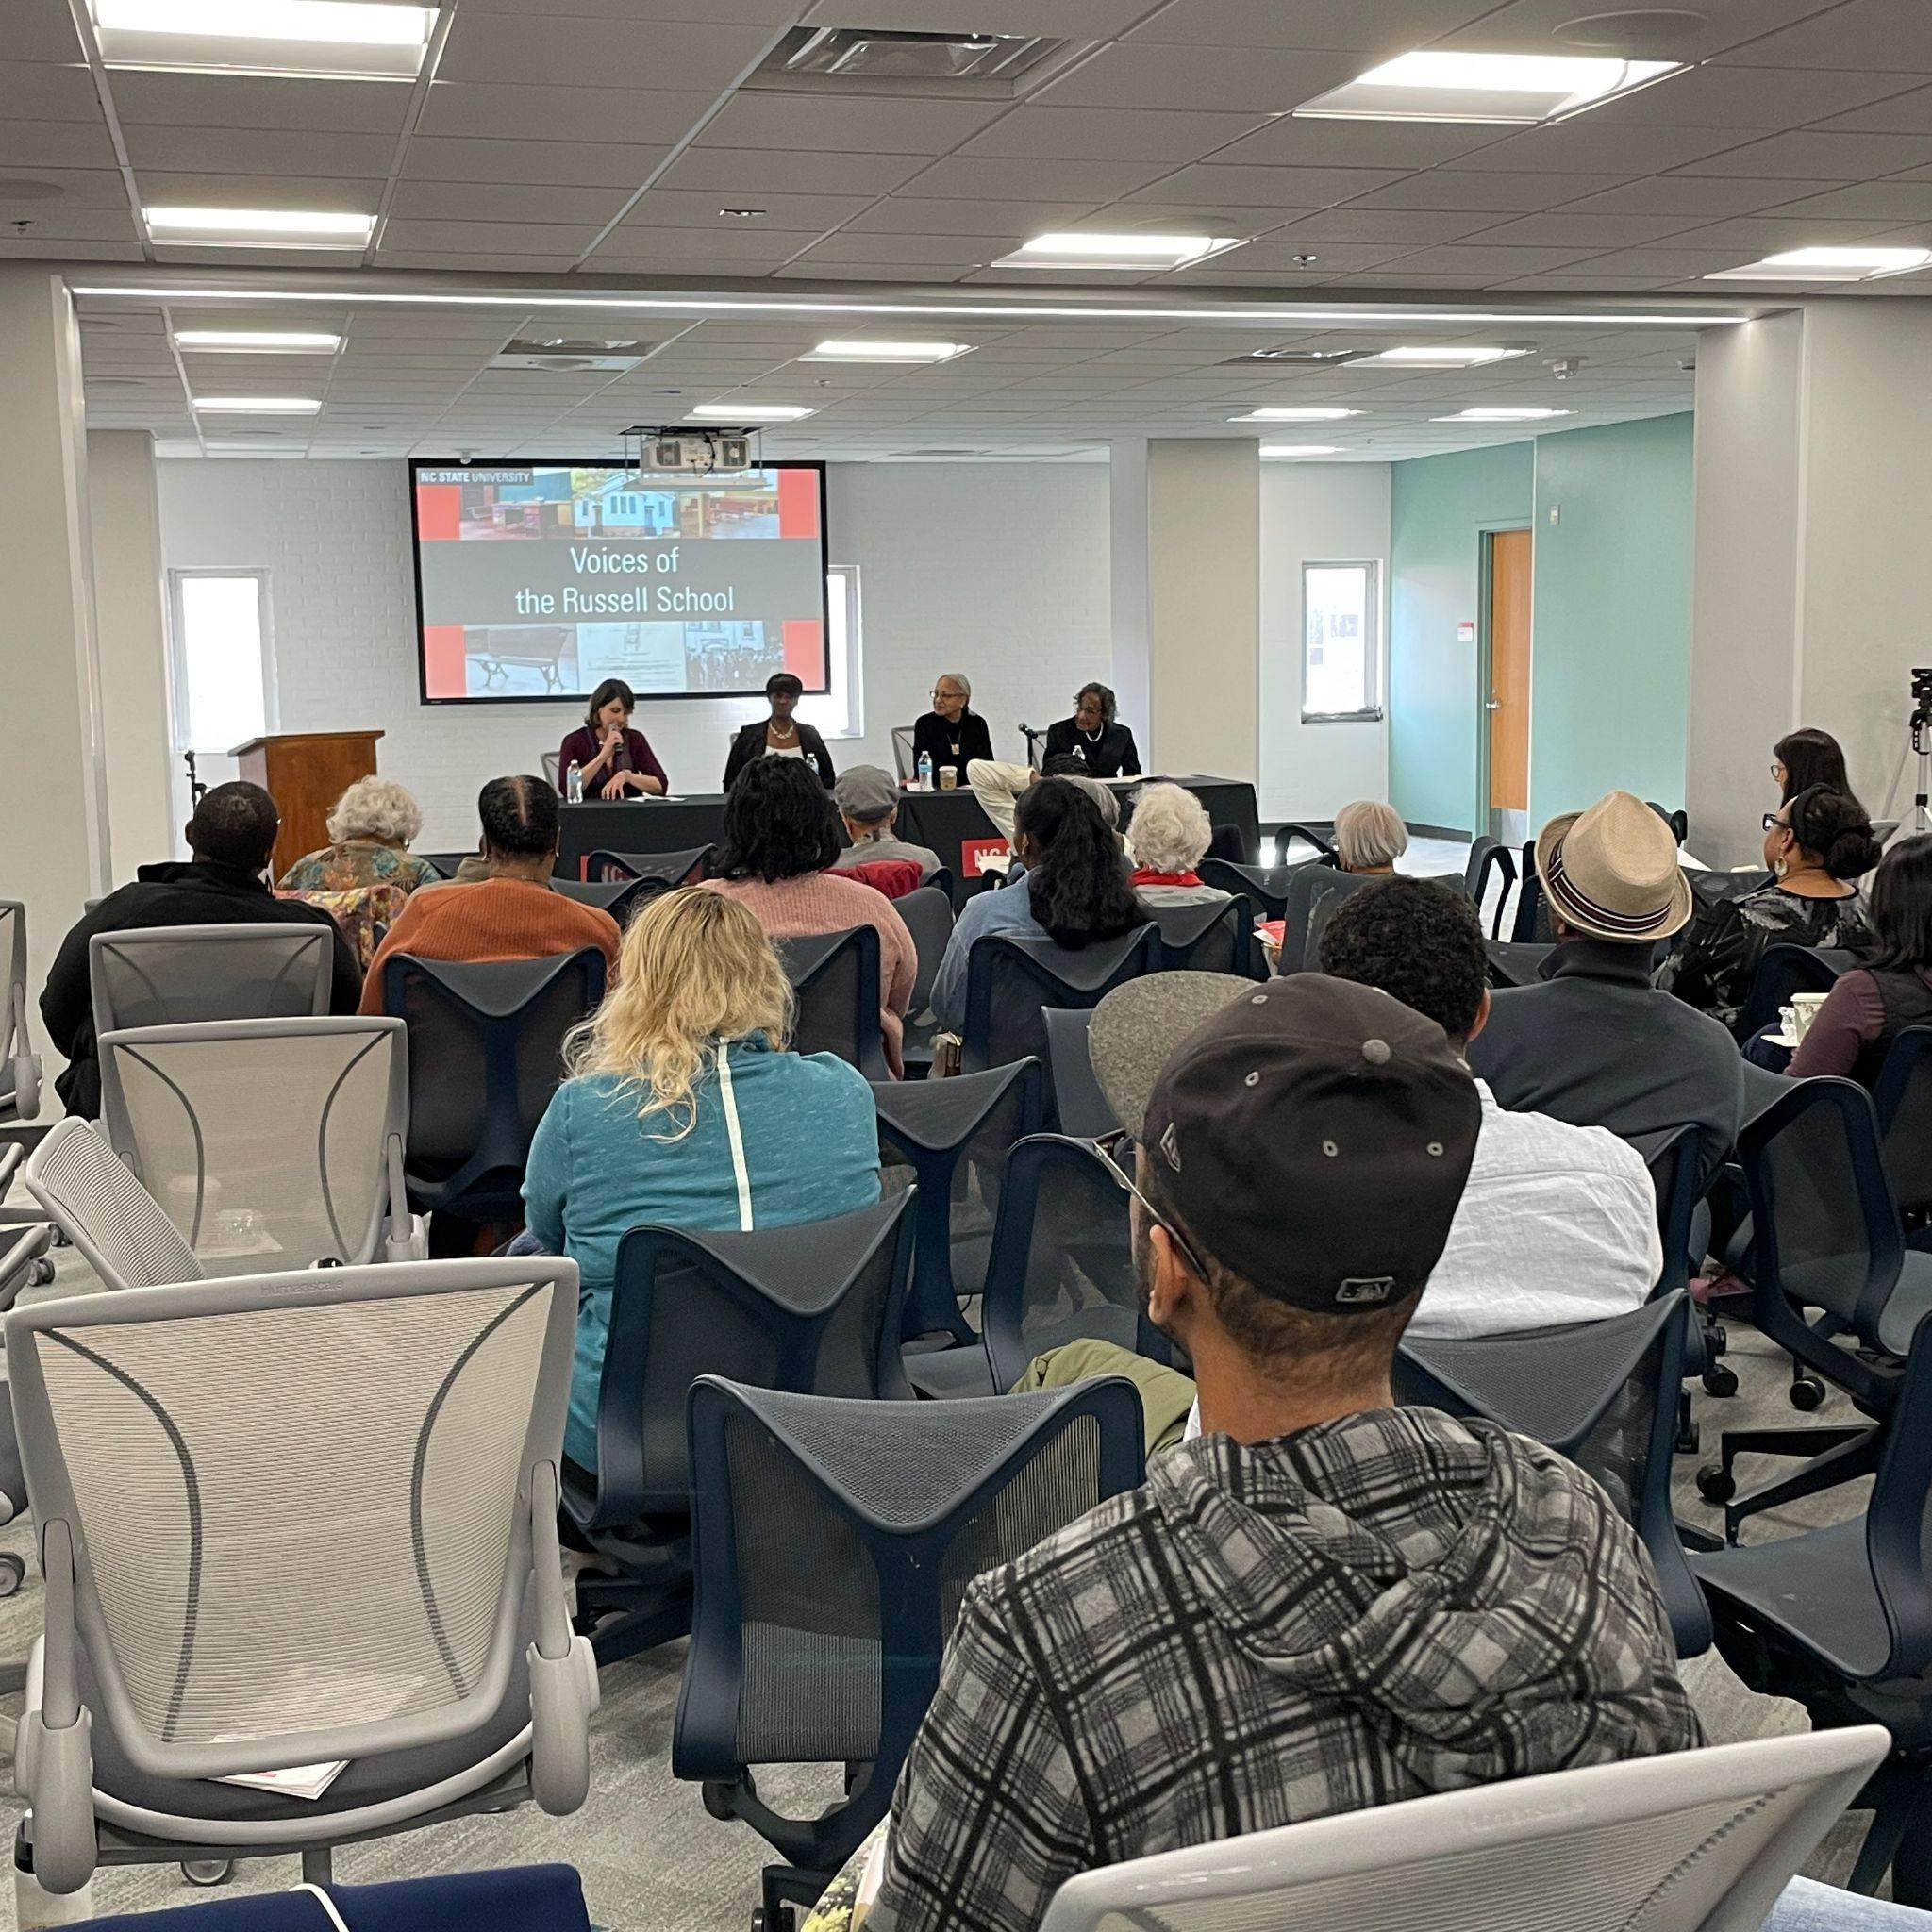
\includegraphics[width=0.6\linewidth]{images/figure1.jpg}
  \caption{Panel Discussion in D.H. Hill Library at NC State University.}
  \label{fig:panel}
\end{figure}

The immersive, museum-style learning experience at the university's D.H. Hill Library was designed with a clear pedagogical purpose: to illuminate historic educational inequities through storytelling for the campus community, the Russell School community, and the general public. This learning environment was intentionally constructed to achieve a deepened understanding of U.S. American educational disparities, their systemic nature, and their impacts. The instructional design followed methodological principles that Morrison et al.\ \cite[p.~142]{morrison2019designing} describe as \enquote{sequences and methods of instruction to achieve an objective,} incorporating spatial narrative techniques, interactive elements, and comparative visual displays to guide learners through a structured examination of educational inequality. By employing sequenced instructional strategies within an immersive context, the experience created opportunities for meaningful, personal engagement with complex social issues that might otherwise remain abstract or disconnected from visitors' lived experiences.

During the design phase, the team focused on creating a coherent visitor journey through the exhibition. As Morrison et al.\ \cite[p.~17]{morrison2019designing} note, sequencing is an important technique that helps learners \enquote{grasp the ideas in a more efficient and effective manner.} This principle applies equally to visitors experiencing an exhibition. The experiences and exhibits were intentionally sequenced to: 1)~\textit{immerse} guests in the Russell School space in case they had not previously visited the structure (VR Studio), 2)~\textit{inspire} guests through compelling narratives and stories (Cyma Rubin Visualization Gallery), and 3)~\textit{connect} guests to the broader Rosenwald Schools story with additional context to explore at one's own pace (iPearl Innovation Studio). This progression meant that each exhibit did not need to tell the entire story of the Russell School; each piece was meant to be seen in combination with the others, creating a full picture of the materials. Event planners noted the progression of most guests from micro-level details about a single school in immersive experiences to macro-level details about the broader Rosenwald Schools program in digital exhibits worked effectively to contextualize locally what guests would discover about the broader movement.

\section{Constructing the Matterport Virtual Tour for Web-Based Use}

DELTA provided technical assistance to capture 360-degree images inside and outside the Russell School using Matterport equipment, while faculty worked with the Friends of Russell Rosenwald School Board to schedule and capture interview footage of community members and school alumni discussing physical elements of the school and the importance of the school to their families and community. Raw interview footage was reviewed, coded, and re-sorted into a themed cut list with time stamps to aid a graduate student with splicing clips from say three to four different interviewees into a single combined clip. This initial coding and organization of the video content formed the foundation for the didactic approach used in designing the exhibit. The analysis revealed several key themes, including the importance of specific locations inside and around the school, community connections, and the impact of educational inequity on students' experiences.

Edited clips were ultimately posted on Youtube, a shareable platform from which video clips could be referenced and opened within the Matterport tour which also provided for auto-captioning (full video playlist available at \url{https://www.youtube.com/playlist?list=PL7XqD5YKzB1651pPT_MyTdnKTWRAMAcF5}). DELTA worked with faculty to finalize the virtual tour by setting up interactive hot spots within Matterport scenes where faculty wanted to emphasize content elements, and by providing a Google Slides template to curate pop-up content (text, images, embedded Youtube video) that displays when viewers click particular hot spots within the tour. The completed virtual tour and embedded content can be viewed at: \url{https://go.ncsu.edu/russell.school}.

\begin{figure}[t!]
  \centering
  
\includegraphics[width=0.7\linewidth]{images/figure2.png}
  \caption{Matterport Virtual Tour Showing Opaque Navigation Jumps and Solid Hot Spots to Open Content.}
  \label{fig:matterport}
\end{figure}

\section{Constructing the Immersive Tours for On-Campus Use}

\subsection{Immersive Tour on VR Headsets}

The library event was open to the university community, Russell School community, and general public, many of whom had never visited the physical Russell School and may not have viewed the Matterport virtual tour either. To provide guests with a better sense of the Russell School as a sample two-room Rosenwald School, Matterport images were exported and merged with interview audio, focusing specifically on introducing the physical features of the school (chalkboards, podium, windows, room divider). To plan for this virtual walk-through, a table was created noting the scenes to feature, the 360-degree image to display at each scene, and the audio clip to play while that scene was displayed, with 14 stops ultimately planned.

Given the divergent age ranges and technical expertise expected of event attendees, a decision was made to auto-walk users through the space with views extracted from 360-degree images and audio clips extracted from interview segments playing back on a defined timeline. The team was concerned that free exploration like that in the original Matterport tour could confuse some participants unfamiliar with hand-mounted controls to virtually navigate school scenes. Users could still rotate their chair or head to see the full 360-degree view, but did not have to move from waypoint to waypoint. DELTA and the library's VR Studio (\url{https://www.lib.ncsu.edu/spaces/gaming-and-vr-studio}) provided expertise and equipment on the day of the public event to assist users with activating the tour that had been pre-loaded on headsets.

\begin{figure}[t!]
  \centering
  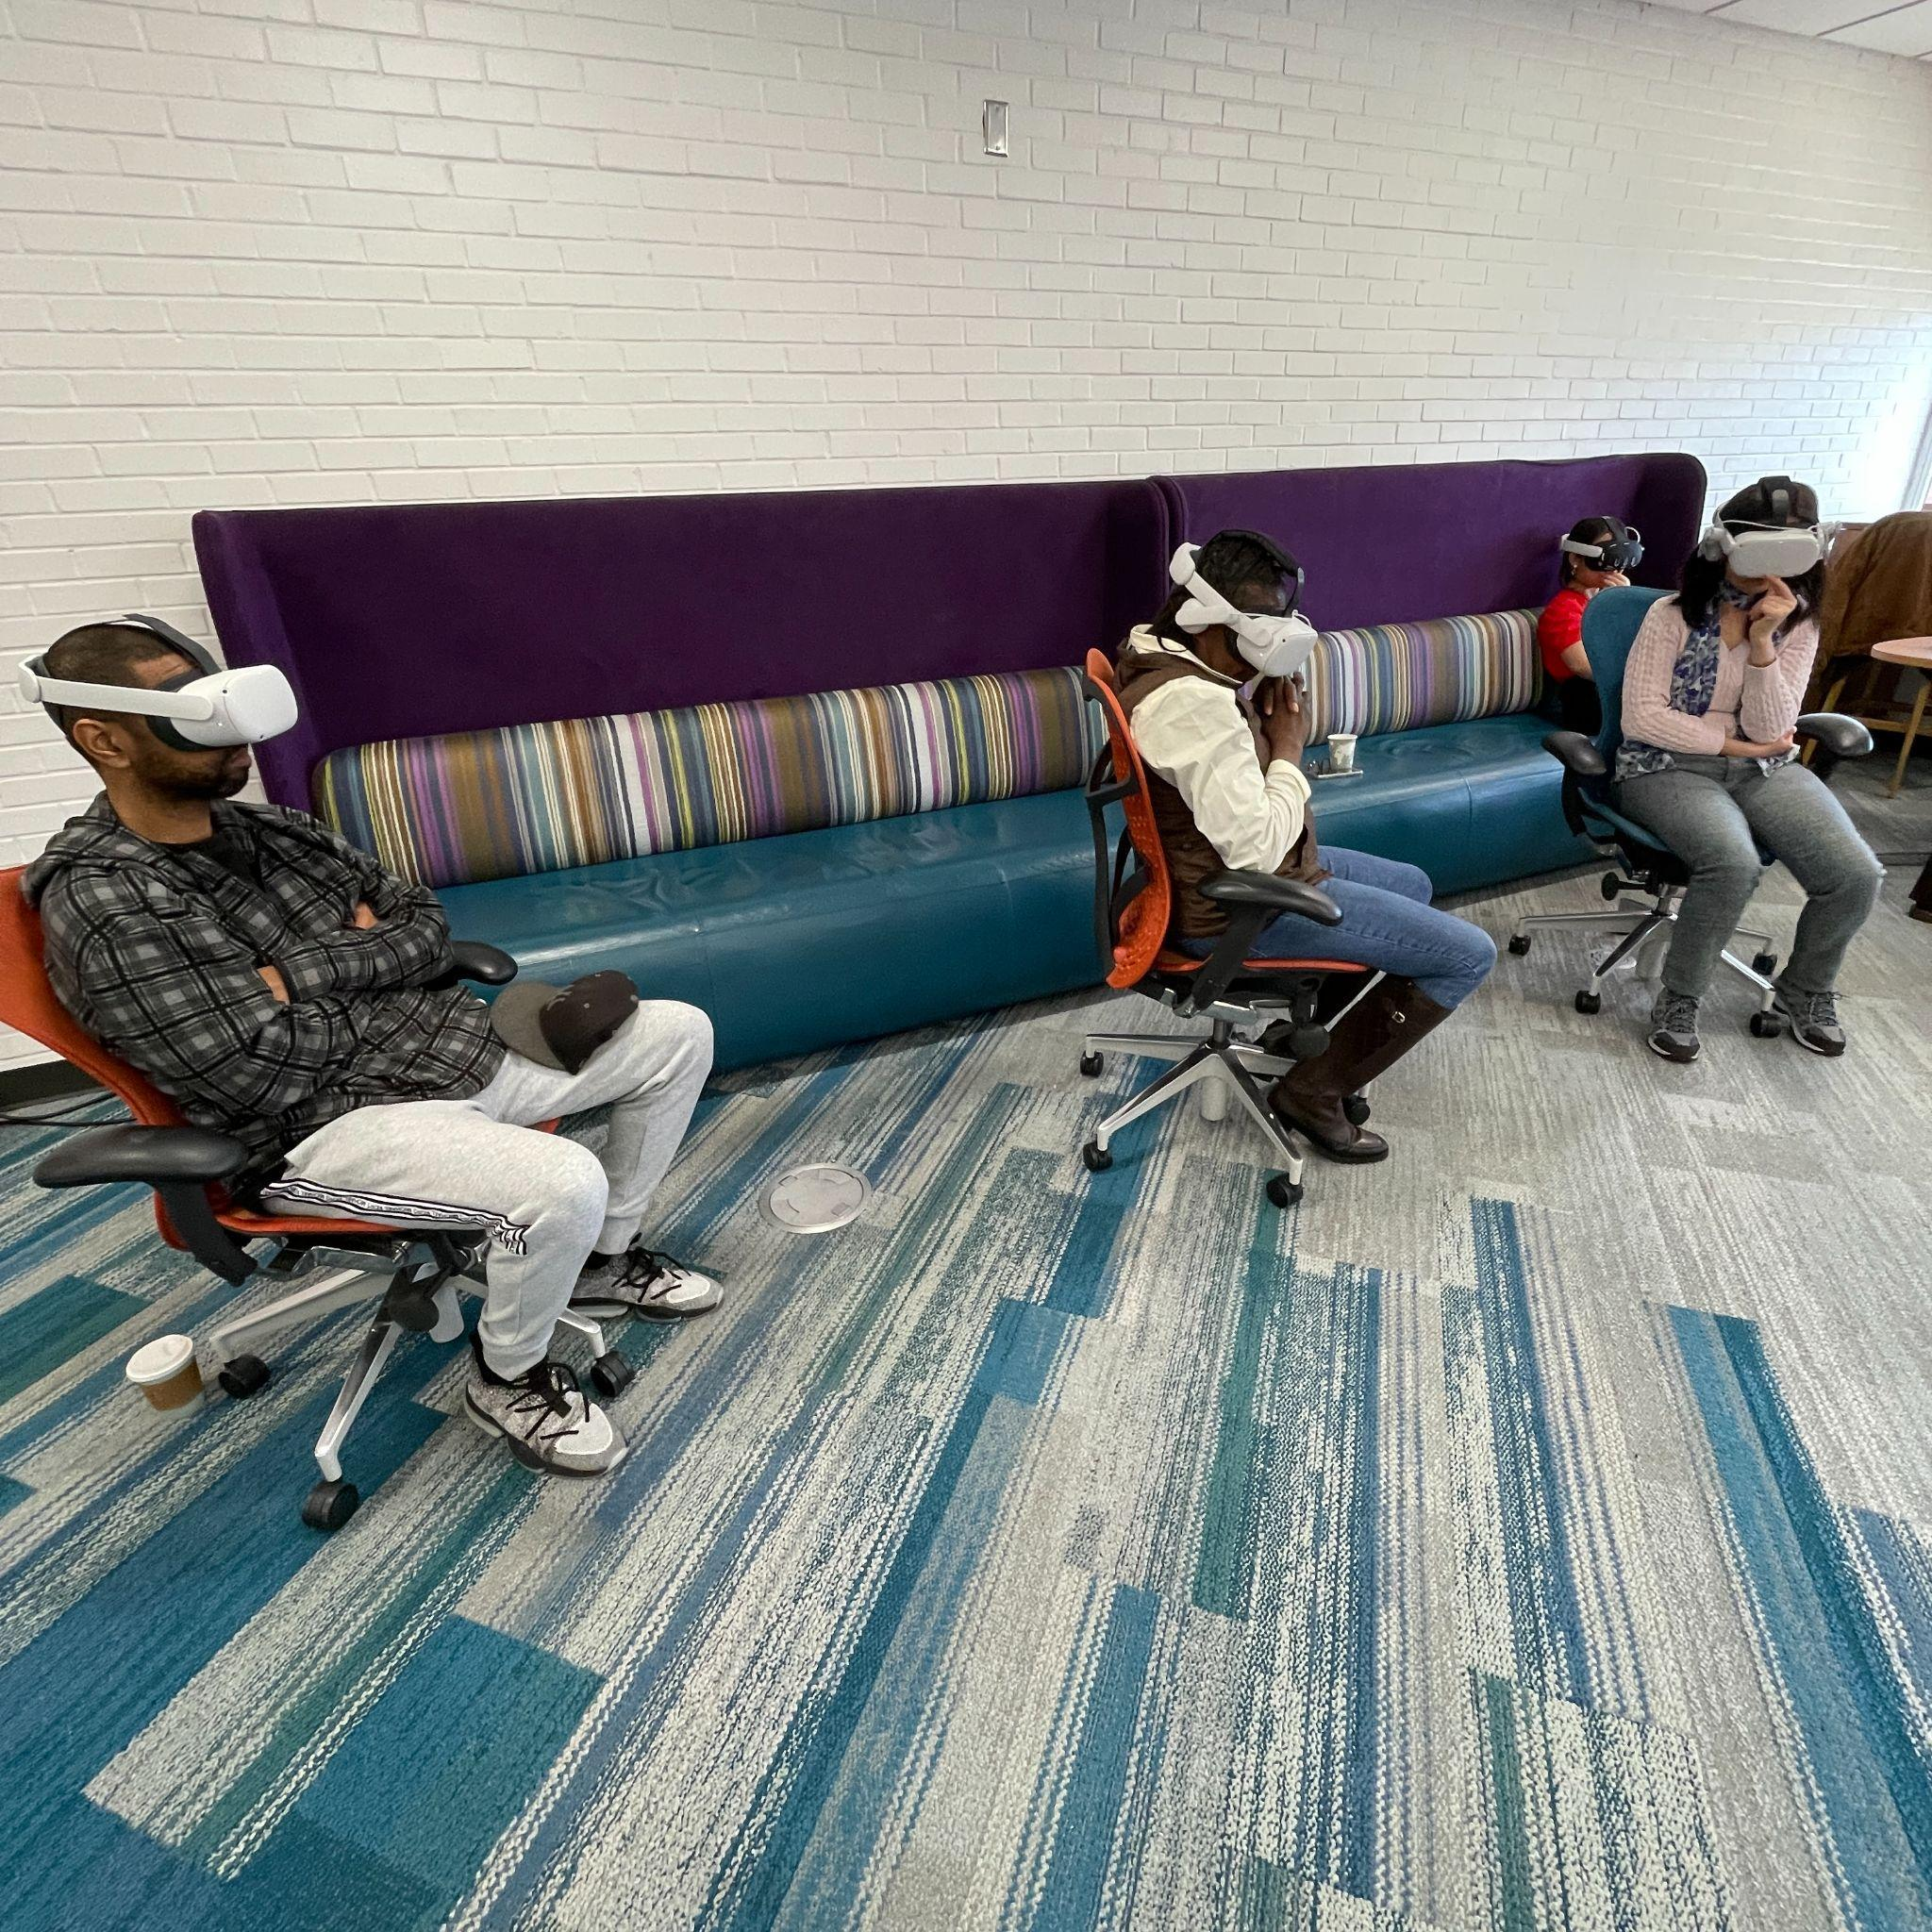
\includegraphics[width=0.6\linewidth]{images/figure3.jpg}
  \caption{Event Guests Viewing the Immersive Tour on Virtual Reality Headsets.}
  \label{fig:vr-headsets}
\end{figure}

\subsection{Immersive 360-Degree Gallery Space}

Whereas VR headsets were used for immersion and introducing physical school features, the theatrical qualities inherent in the library's 360-degree Cyma Rubin Visualization Gallery (\url{https://www.lib.ncsu.edu/spaces/cyma-rubin-visualization-gallery}) lent themselves to inspiring guests by panning up into one's full view both external and internal school scenes (also exported from original Matterport images), cueing compelling interview segments to display over the scenes, and merging appropriate music including a joyful hymn recorded in and provided by the church that owns and maintains the adjacent Russell School. The gallery offers a seamless 360-degree visual landscape with a display resolution of 15,360 $\times$ 1080 pixels in total. Spanning 27.5 feet across, this gallery utilizes state-of-the-art equipment, including eight high-definition projectors. A standard stereo setup was used for this project, though the studio is equipped with 7.1 surround sound and stereo audio systems.

Matterport images, initially tailored for interactive 3D or Virtual Reality applications, underwent adjustments in Adobe Photoshop to align with flat 360 screens. Using generative fill and copying techniques, the images were warped and extended, yet with some residual skewing in certain areas. For example, the main focus object of one scene, a building, still resembled a photograph with a fish eye lens after edits. Additionally, AI-based upscaling and sharpening were applied to the Matterport images, leading to a slightly stylized, illustrative quality. To enhance this effect, color adjustments, posterization, and line effects were added in Photoshop. Additionally, imperfections such as a forgotten camera in the background, other artifacts, scratches on the board, and other elements were removed. Subsequently, interviews and backgrounds were imported into Adobe After Effects for video editing and cutting. The editing workload was barely managed by a MacBook Pro Retina equipped with an Intel Core i7 processor and an NVIDIA GeForce GT 750M 2 GB graphics card. Even previewing the project within After Effects was impossible without rendering a small draft. Hence, the rendering processes were outsourced to an external rendering machine with two graphics cards. The libraries provided a stretched Google Slides template to import the finished video for display in the gallery. It took more than five testing rounds to gap the difference between projector and computer screen, for example for the elevated contrast and brightness of the projectors, the size of elements on screen in relation to the viewer's distance to the screen, speed of animations, and video cut types.

\begin{figure}[t!]
  \centering
  
\includegraphics[width=0.6\linewidth]{images/figure4.png}
  \caption{Event Guests Viewing the 360-Degree Video in the Visualization Gallery.}
  \label{fig:gallery}
\end{figure}

\section{Constructing the Digital Exhibits}

Studio exhibits were used during the event to connect the Russell School story with other Rosenwald Schools through archival material. The library's iPearl Innovation Studio (\url{https://www.lib.ncsu.edu/spaces/ipearl-innovation-studio}) contains eight custom-built interactive projection tables on which visitors can browse through exhibit content using gesture-based navigation with their hands. Faculty planned eight exhibits for these tables drawing on existing digital materials (e.g., archival photographs on Rosenwald Schools from the State Archives of North Carolina, maps illustrating remaining Rosenwald Schools in the state curated by the Division of Natural and Cultural Resources, published Rosenwald School floor plans from the Rosenwald Fund, published Omeka collections on related topics like Rosenwald's broader philanthropy to support artists, selected interview footage collected for the original virtual tour) and some physical materials (e.g., showcased children's literature on Rosenwald Schools). A scavenger hunt was prepared for this space to encourage visitors to spend time reading/viewing the different exhibits in order to answer all of the questions on the handout.

\begin{figure}[t!]
  \centering
  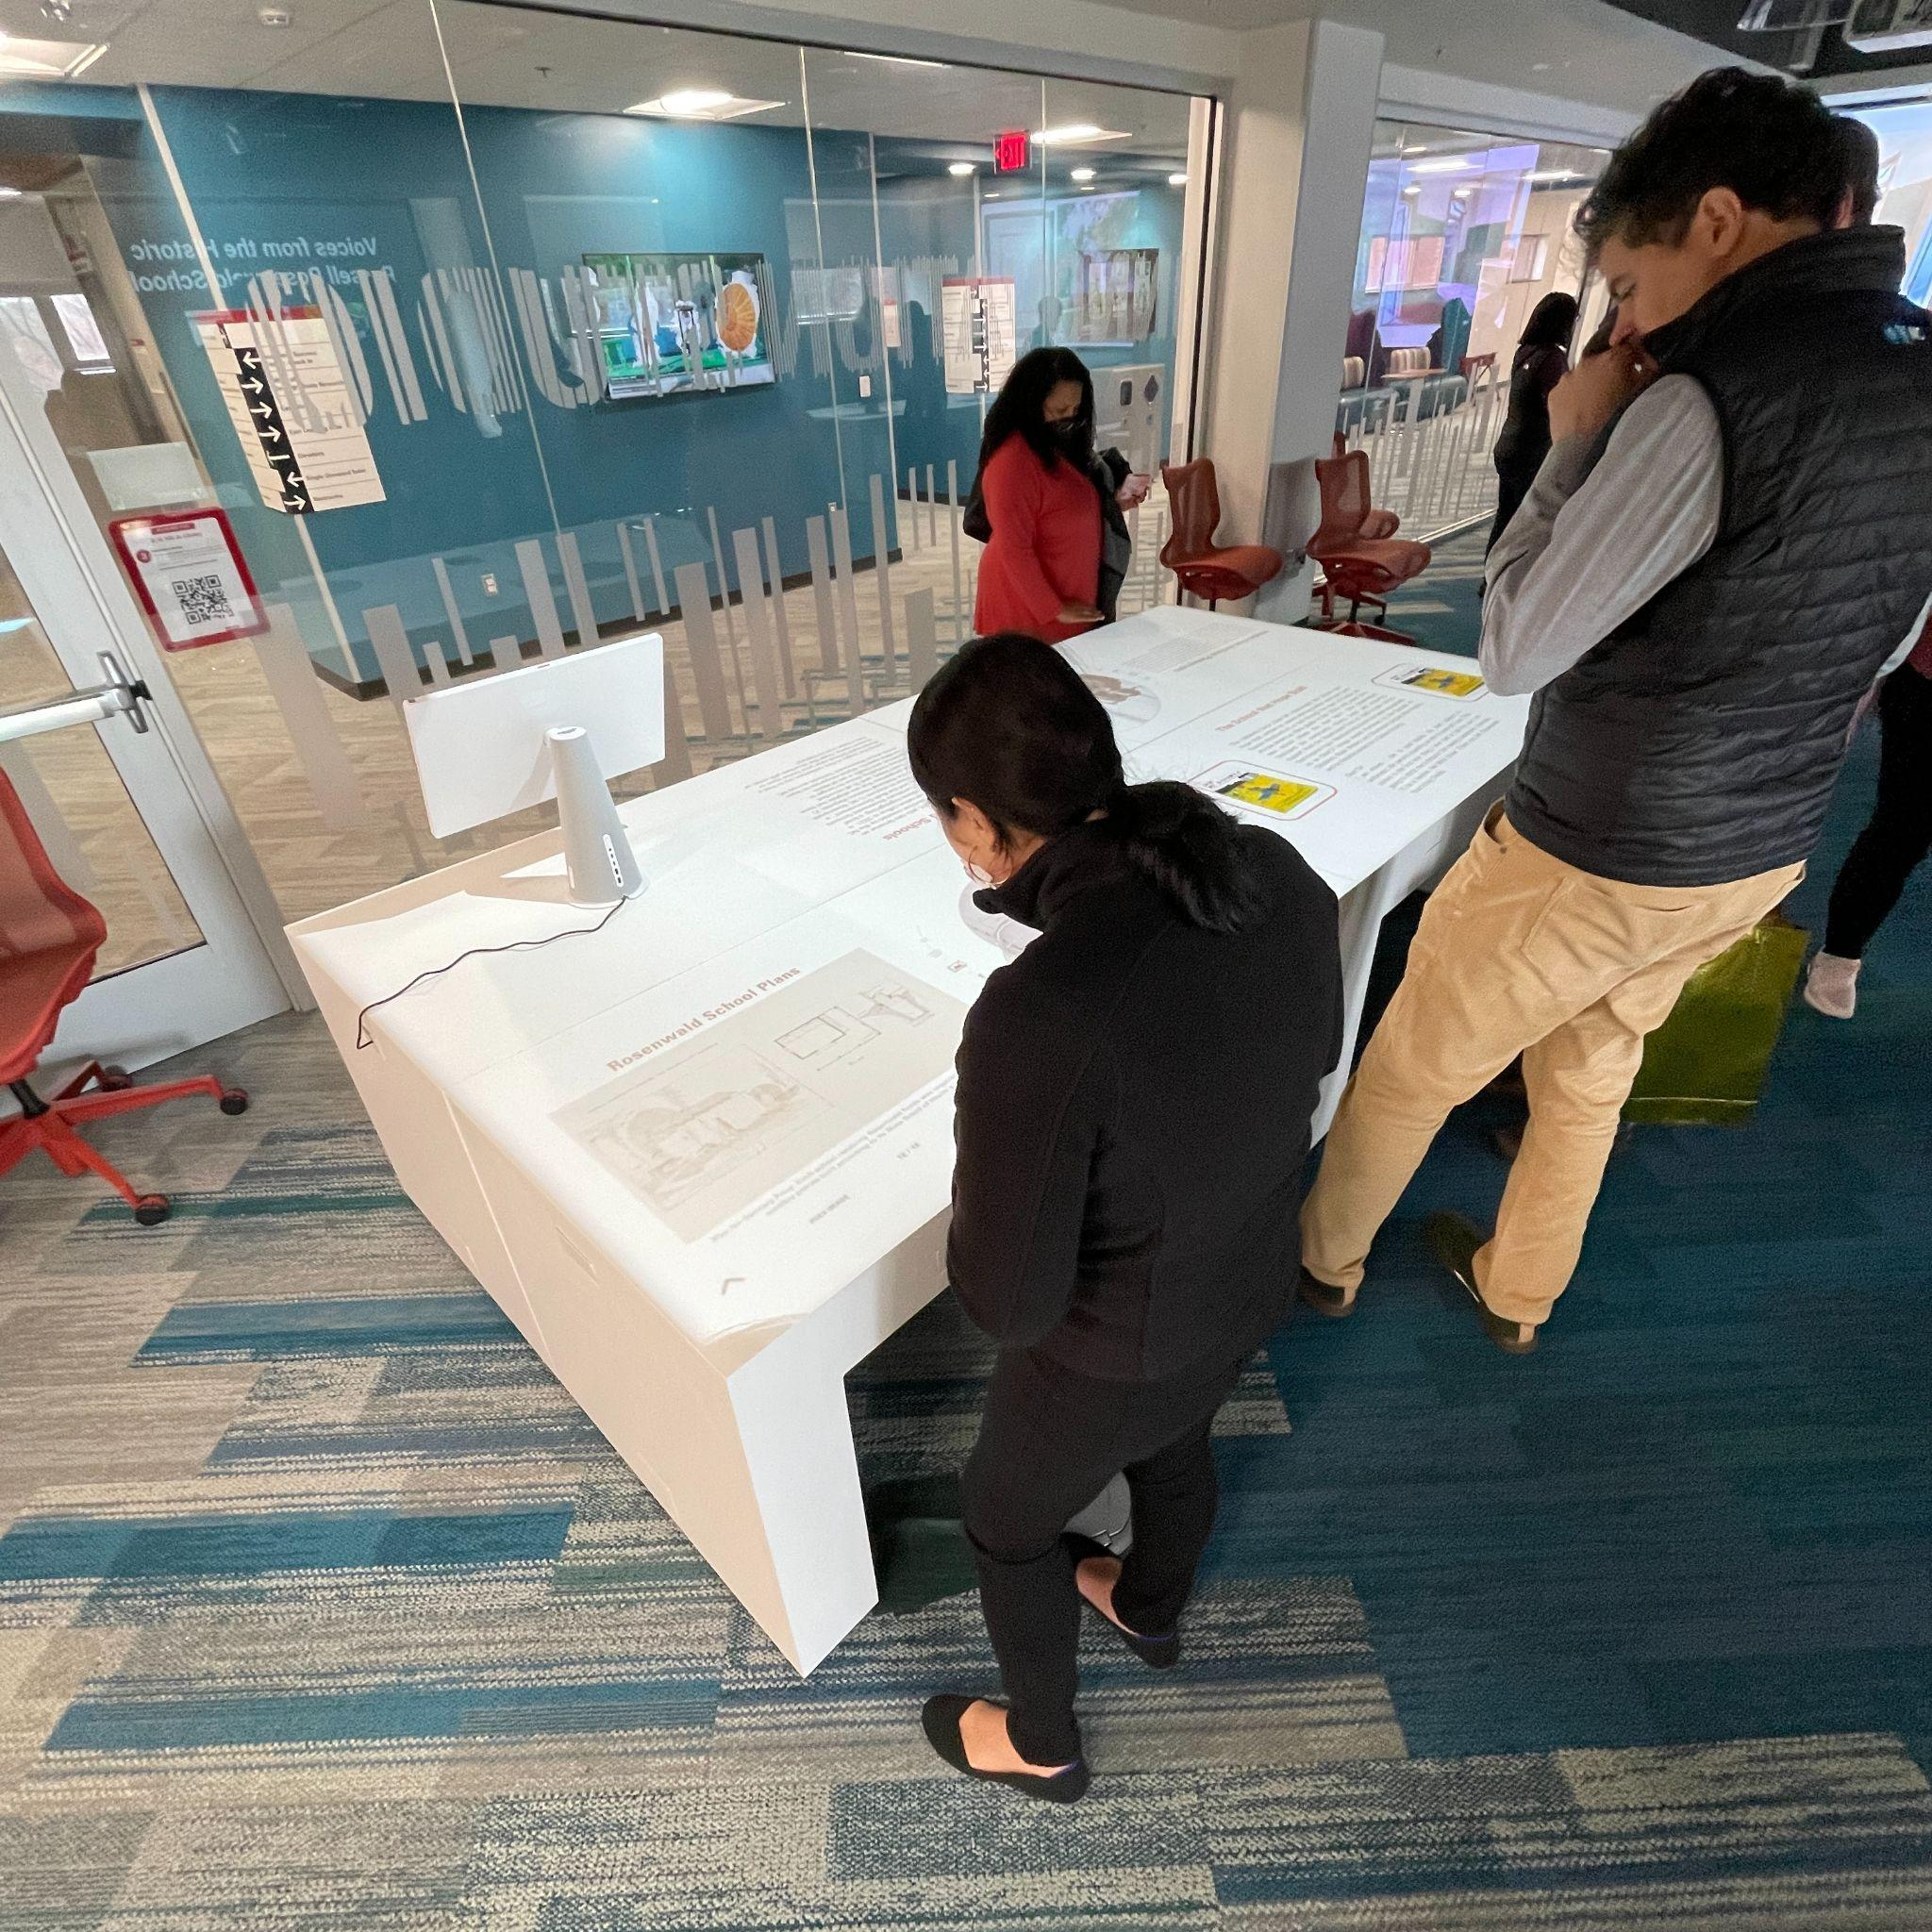
\includegraphics[width=0.6\linewidth]{images/figure5.jpg}
  \caption{Event Guests Viewing Digital Exhibits in the Innovation Studio.}
  \label{fig:exhibits}
\end{figure}

\section{Event Management and Impact}

To carry off the public event in this project required the participation of numerous persons. Beyond the broader team that technically designed and produced exhibits as described above, the College of Education donated its van to pick up elderly guests from the Russell School community and bring them to the event. The state chapter of the Fulbright Association co-sponsored the event and provided funding for campus-catered food and drinks. College of Education student ambassadors greeted and directed visitors to the panel and different event spaces spread between two library floors. DELTA and libraries staff provided technical support on the day of the event to ensure microphones worked for panelists and event spaces functioned properly.

Evidence of event impact falls into two categories---networking and capacity building. First, faculty and librarians supporting the project were able to effectively network with Rosenwald School community groups and cultural heritage enthusiasts through the event. During the event, faculty spoke with representatives of further Rosenwald Schools in the area with whom they might collaborate on future projects, and these school groups were able to meet with and learn from one another such as steps taken by the Russell School to create virtual resources to further their education mission. Further, our academic panelist on Rosenwald Schools from South Carolina reached out to the libraries after the event and asked if we might reprise the event spaces for a group of government officials from her state. Faculty and librarians did meet with this group to screen the exhibits we had created and discussed opportunities to represent Rosenwald Schools in their state through similar facilities and exhibits. In terms of capacity building, research for this project has already assisted faculty with proposing follow-on external grants in the area of digital cultural heritage of Rosenwald Schools. One early success is a small grant and technical assistance received from the non-profit group Cyark who visited the Russell School in 2026 to capture their own 360-degree images and interview footage for a separate Tapestry virtual experience on the broader Rosenwald Schools movement. This follow-on multimedia experience was released as part of America 250 celebrations and the Russell School's centennial anniversary.

One of the many potentials of immersive technologies is to preserve, display, and present historic sites to a wider audience. In this case, we planned and showed an immersive exhibition to share the voices of contemporary eyewitnesses who attended a local Rosenwald school through virtual reality headsets, a 360-degree film, and interactive touchless tables. By framing the exhibit with a panel discussion, the local community introduced the impact of Rosenwald's local legacy on their lives. We found that interacting with immersive spaces is a viable means for all ages to evoke interest and support exploring physical spaces. We propose that multi-form immersion is a useful way to preserve and share the history in historic sites.

\printbibliography

\end{document}
